\documentclass[12pt,letterpaper,twoside]{book}
%- - - - - - - - - - - - - - - - - - - - - -- - - - - - - - - - 
%            Pre�mbulo del documento. Configuraciones varias
%- - - - - - - - - - - - - - - - - - - - - - - - - - - - - - - - 
\usepackage[most]{tcolorbox}
\usepackage{acronym}
\usepackage{multirow} 
\usepackage{array}
\usepackage{booktabs}
\usepackage{threeparttable}
\usepackage{url}
\usepackage{pbox}
\usepackage{makecell}
\usepackage{multirow}
\usepackage{float}
\usepackage{amssymb}
\usepackage{amsmath}
\usepackage{rotating}
\usepackage{geometry}
\geometry{bindingoffset=2cm}
\geometry{textwidth=360pt}
\usepackage{pdfpages}
\usepackage{anysize}
\usepackage{TeXiS/TeXiS}
\hypersetup{%
	pdftitle = {T�tulo},
   pdfsubject = {Tesis de Mestr�a SEPI Telecomunicaciones ESIME Zacatenco},
   pdfkeywords = {},
   pdfauthor = {\textcopyright\ Autor},
   pdfcreator = {\LaTeX\ con el paquete \flqq hyperref\frqq},
   pdfproducer = {pdfeTeX-0.\the\pdftexversion\pdftexrevision},
   }
    \pdfinfo{/CreationDate (\today)}
\papersize{27.9cm}{21.5cm} 
\marginsize{2.5cm}{2.5cm}{1.5cm}{2.5cm}
\usepackage[export]{adjustbox}
\usepackage{mathptmx}
\usepackage{setspace}
\usepackage{siunitx}
\usepackage{csquotes}
\usepackage[backend=bibtex,refsegment=chapter, style=ieee]{biblatex}
\addbibresource{referencias.bib}
\AtBeginBibliography{\footnotesize}
\usepackage{caption}
\captionsetup{font=small}
\begin{document}
\renewcommand{\bibname}{Referencias}
\frontmatter
\spacing{1.3}
\definecolor{coloripn}{RGB}{112,29,69}
\thispagestyle{empty} 
\hspace{-1cm}\begin{minipage}[c][0.12\textheight][c]{0.14\textwidth}
    \begin{center}
        \includegraphics[height=4cm, keepaspectratio=true]{fig/logoipn} %% LOGO IZQUIERDO
    \end{center}
\end{minipage}
\hspace{0.7cm}
\begin{minipage}[c][0.17\textheight][t]{0.7\textwidth}
    \begin{center}
        {\scshape \Huge Instituto Polit�cnico Nacional} %% NOMBRE DE LA UNIVERSIDAD
        \vspace{.5cm}   %% DEFINE EL ESPACIO ENTRE EL NOMBRE DE LA UNIVERSIDAD Y LA L�NEA DOBLE
       {\color{coloripn}  \hrule height2.5pt}  %% DEFINE EL ANCHO DE LA PRIMER L�NEA
        \vspace{.1cm}    %% DEFINE EL ESPACIO ENTRE LAS DOS LINEAS
       {\color{coloripn} \hrule height1pt}  %% DEFINE EL ANCHO DE LA SEGUNDA LINEA (NORMALMENTE ES MAS DELGADA)
        \vspace{.4cm}   %% DEFINE EL ESPACIO ENTRE LA DOBLE LINEA Y EL NOMBRE DE LA DIVISI�N
        {\scshape \Large Escuela Superior de Ingenier�a Mec�nica y El�ctrica}  %% NOMBRE DE LA DIVISI�N
        %\vspace{.1cm}  
        
        {\scshape \large Unidad Profesional Adolfo L�pez Mateos}
        
        \vspace{.4cm}  
        
        {\scshape \Large Secci�n de Estudios de Posgrado e Investigaci�n}
    \end{center}
\end{minipage}
\begin{minipage}[c][0.12\textheight][c]{0.14\textwidth}
    \begin{center}
        
\includegraphics[height=2.5cm, keepaspectratio=true]{fig/logoesime}  %% DEFINIR EL ARCHIVO O RUTA DEL LOGO DERECHO
    \end{center}
\end{minipage}
%}
%
%
%
%
%
%    ESPACIO COMENTADO PARA EVITAR DESAJUSTES POR GENERACI�N DE NUEVO P�RRAFO (NO DEJAR ESPACIOS ENTRE MINIPAGES)
%
%
%
%
%
%
%%%%%%% RENGL�N DE ABAJO DEJADO INTENCIONALMENTE EN BLANCO PARA GENERAR NUEVO COMIENZO DE P�RRAFO  %%%%%%

%%%%%%%%%%%%%%%%%%%%%%%%%%%%%%%%%%%%%%%%%%%%%%%%%%%%%%%%%%%%%%%%%%%%%%%%%%%%%%%%%%%%%%%%%%%%%%%%%%%%%%%%%
%
%
%
%
%
%  ESPACIO COMENTADO PARA EVITAR DESAJUSTES POR GENERACI�N DE NUEVO P�RRAFO (NO DEJAR ESPACIOS ENTRE MINIPAGES)
%
%
%
%
%
%
%%%%%%%%%%%%%%%% 5TO MINIPAGE PARA EL CUERPO DE LA PORTADA (NOMBRES, T�TULO, ETC.) %%%%%%%%%%%%%%%%%%%%%%%%%%%%%%%%%%%%%%
%
%
%
%
%\fbox{
\begin{minipage}[l][0.78\textheight][t]{0.1\textwidth}
    \begin{center}
    \hskip0pt
    {\color{coloripn}\vrule width2.5pt height17cm}    %% height definde la altura de la linea gruesa
        \hskip 0.1cm
        {\color{coloripn}\vrule width1pt height17cm } %% height define la altura de la linea delgada
        \end{center}
\end{minipage}
%}
%\fbox{
\begin{minipage}[c][0.78\textheight][t]{0.8\textwidth}
      \begin{center}
      \vspace{3cm}
        {\large \scshape {T�tulo del trabajo de tesis}}

        \vspace{0.5cm}

        \makebox[5cm][c]{\Large TESIS} 
        
        \vspace{0.5cm}
        
        {\large Que para obtener el grado de:}\\
        
        \large {XXXXX en Ciencias en Ingenier�a de Telecomunicaciones}
        \vspace{0.5cm}
        
        {\large Presenta:}\\
     
        \large {Nombre}

        \vspace{0.5cm}

        { \large Directores}:\\ {\large Dr. XXXXX \\ Dr. XXXXX}

        \vspace{1.3cm}

        {\large Ciudad de M�xico} \hskip2.3cm {\large \today}
      \end{center}
\end{minipage}

\newpage
% Segunda p�gina, vacia
\thispagestyle{empty}\mbox{}
\newpage
%}

La plantilla est� basada en TeXiS: \url{http://gaia.fdi.ucm.es/research/texis/} por lo que se recomienda consultar su manual. TeXiS se distribuye bajo las licencias \LaTeX\ Project Public License (Licencia P�blica del Proyecto \LaTeX), GPLv3 y Creative Commons (CC-BY-SA). \\ \\
El documento ya est� preparado para ser impreso a doble cara. 
%--------------------------------------------------------
%				Contiene la p�gina de dedicatorias.
%--------------------------------------------------------
\dedicatoriaUno{
\emph{
Dedicatoria
}
}
\makeDedicatorias

%--------------------------------------------------------
%                      agradecimientos.tex
% 			Contiene la p�gina de agradecimientos.
% 			Se crea como un cap�tulo sin numeraci�n.
%--------------------------------------------------------
\chapter{Agradecimientos}
\cabeceraEspecial{Agradecimientos}


\endinput

\include{Cascaras/resumen}
\include{Cascaras/abstract}
\include{Cascaras/estructura}
%---------------------------------------------------------------------
%
%                          TeXiS_toc.tex
%
%---------------------------------------------------------------------
%
% TeXiS_toc.tex
% Copyright 2009 Marco Antonio Gomez-Martin, Pedro Pablo Gomez-Martin
%
% This file belongs to TeXiS, a LaTeX template for writting
% Thesis and other documents. The complete last TeXiS package can
% be obtained from http://gaia.fdi.ucm.es/projects/texis/
%
% This work may be distributed and/or modified under the
% conditions of the LaTeX Project Public License, either version 1.3
% of this license or (at your option) any later version.
% The latest version of this license is in
%   http://www.latex-project.org/lppl.txt
% and version 1.3 or later is part of all distributions of LaTeX
% version 2005/12/01 or later.
%
% This work has the LPPL maintenance status `maintained'.
% 
% The Current Maintainers of this work are Marco Antonio Gomez-Martin
% and Pedro Pablo Gomez-Martin
%
%---------------------------------------------------------------------
%
% Contiene  los  comandos  para  generar los  �ndices  del  documento,
% entendiendo por �ndices las tablas de contenidos.
%
% Genera  el  �ndice normal  ("tabla  de  contenidos"),  el �ndice  de
% figuras y el de tablas. Tambi�n  crea "marcadores" en el caso de que
% se est� compilando con pdflatex para que aparezcan en el PDF.
%
%---------------------------------------------------------------------


% Primero un poquito de configuraci�n...


% Pedimos que inserte todos los ep�grafes hasta el nivel \subsection en
% la tabla de contenidos.
\setcounter{tocdepth}{2} 

% Le  pedimos  que nos  numere  todos  los  ep�grafes hasta  el  nivel
% \subsubsection en el cuerpo del documento.
\setcounter{secnumdepth}{3} 


% Creamos los diferentes �ndices.

% Lo primero un  poco de trabajo en los marcadores  del PDF. No quiero
% que  salga una  entrada  por cada  �ndice  a nivel  0...  si no  que
% aparezca un marcador "�ndices", que  tenga dentro los otros tipos de
% �ndices.  Total, que creamos el marcador "�ndices".
% Antes de  la creaci�n  de los �ndices,  se a�aden los  marcadores de
% nivel 1.

\ifpdf
   \pdfbookmark{�ndices}{indices}
\fi

% Tabla de contenidos.
%
% La  inclusi�n  de '\tableofcontents'  significa  que  en la  primera
% pasada  de  LaTeX  se  crea   un  fichero  con  extensi�n  .toc  con
% informaci�n sobre la tabla de contenidos (es conceptualmente similar
% al  .bbl de  BibTeX, creo).  En la  segunda ejecuci�n  de  LaTeX ese
% documento se utiliza para  generar la verdadera p�gina de contenidos
% usando la  informaci�n sobre los  cap�tulos y dem�s guardadas  en el
% .toc
\ifpdf
   \pdfbookmark[1]{Tabla de contenidos}{tabla de contenidos}
\fi

\cabeceraEspecial{\'Indice}

\tableofcontents

\newpage

% �ndice de figuras
%
% La idea es semejante que para  el .toc del �ndice, pero ahora se usa
% extensi�n .lof (List Of Figures) con la informaci�n de las figuras.
\cabeceraEspecial{\'Indice de figuras}

\ifpdf
   \pdfbookmark[1]{�ndice de figuras}{indice de figuras}
\fi
\addcontentsline{toc}{chapter}{�ndice de figuras}
\listoffigures


\newpage

% �ndice de tablas
% Como antes, pero ahora .lot (List Of Tables)

\ifpdf
   \pdfbookmark[1]{�ndice de tablas}{indice de tablas}
\fi

\cabeceraEspecial{\'Indice de tablas}
\addcontentsline{toc}{chapter}{�ndice de tablas}
\listoftables
\newpage


% Variable local para emacs, para  que encuentre el fichero maestro de
% compilaci�n y funcionen mejor algunas teclas r�pidas de AucTeX

%%%
%%% Local Variables:
%%% mode: latex
%%% TeX-master: "../Tesis.tex"
%%% End:

\mainmatter
\restauraCabecera
%---------------------------------------------------------------------
%                          Cap�tulo 1
%---------------------------------------------------------------------
\chapter{Nombre del cap�tulo}
%Etiqueta del cap�tulo	
\label{}
%Estructura para poner una frase c�lebre
\begin{FraseCelebre}
\begin{Frase}
En la vida no existe nada que temer, \\
solo cosas que comprender.
\end{Frase}
\begin{Fuente}
Marie Curie
\end{Fuente}
\end{FraseCelebre}
%-------------------------------------------------------------------
%Aqu� empieza el cap�tulo 
\section{Introducci�n}
Contenido...
\subsection{Contenido...}
Contenido...
\subsubsection{Contenido..}
Contenido...
Ejemplo de cita \cite{RamPac20}.


\begin{figure}
	\centering
	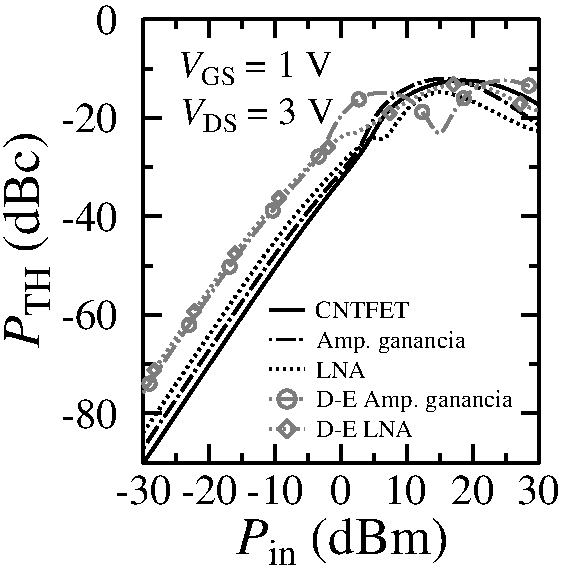
\includegraphics[width=0.45\linewidth]{fig/Capitulo1/Pin_ThirdHarmonic_es}
	\caption{Descripci�n de la figura.}
	\label{fig:pinthirdharmonices}
\end{figure}

Se recomienda al usuario de �sta plantilla utilizar figuras en formato PDF y para generar gr�ficas utilizar el software GLE, un script de ejemplo para generar la Figura \ref{fig:parametrossccamvds3vgs1cntfet} se puede encontrar dentro de la carpeta fig/FuentesCapitulo1.

\begin{figure}
	\centering
	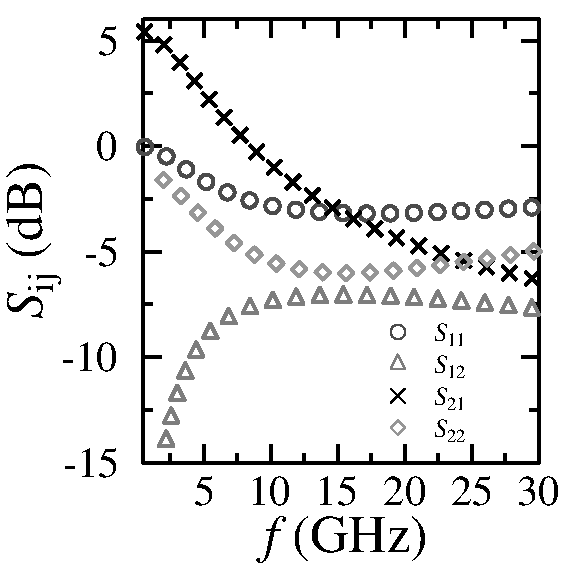
\includegraphics[width=0.45\linewidth]{fig/Capitulo1/Parametros_S_CCAM_VDS_3_VGS_1_CNTFET}
	\caption{Descripci�n de la figura.}
	\label{fig:parametrossccamvds3vgs1cntfet}
\end{figure}


%L�neas para a�adir la bibliograf�a por cada cap�tulo, utilizar bibtex.
\addcontentsline{toc}{chapter}{Referencias}
\printbibliography[segment=\therefsegment]


\endinput


% Ap�ndices
\appendix
%---------------------------------------------------------------------
%
%                          Ap�ndice 1
%
%---------------------------------------------------------------------

\chapter{Nombre del ap�ndice}
\label{}

\begin{FraseCelebre}
\begin{Frase}
	Frase
\end{Frase}
\begin{Fuente}
Fuente
\end{Fuente}
\end{FraseCelebre}

%\begin{resumen}






\backmatter
\include{Cascaras/fin}
\end{document}

